%%%%%%%%%%%%%%%%%%%%%%%%%%%%%%%%%%
\section{Results including photon transverse momentum}
%%%%%%%%%%%%%%%%%%%%%%%%%%%%%%%%%%
%------------------------------------------------------------------------------------

%-------------------------------------------------------------------------------------------
%\subsection{Structure functions as input for unintegrated fluxes}
%-------------------------------------------------------------------------------------------

Several different parametrizations of proton strucure functions are used. Those are labeled as:
%%
\begin{itemize} 

 \item ALLM \cite{Abramowicz:1991xz,Abramowicz:1997ms}: This parametrization gives a good fit to $F_2$ in most of the measured regions.
   
\item FJLLM \cite{Fiore:2002re}: This parametrization explicitly includes the nucleon resonances and provides very good descripton of the CLAS data~\cite{Osipenko:2003bu}.
  
\item SY \cite{Suri:1971yx}: This parameterization of Suri and Yennie from the early 1970's does not include DGLAP evolution. It is still  used as one of the defaults in the LPAIR event generator~\cite{Vermaseren:1982cz}.
    
\item SU \cite{Szczurek:1999rd}: A parametrization which concentrates to give a good description at smal and intermediate $Q^2$ at not too small $x$.
% A Vector-Meson-Dominance model inspired fit of $F_2$ at low $Q^2$, which is 
At large $Q^2$, it is complemented by the NNLO calculation of $F_2$ and $F_L$ from NNLO MSTW 2008 PDF analysis~\cite{Martin:2009iq}.
   
\item LUX-like: a recently constructed parametrization, described in details in Ref.~\cite{Luszczak:2018ntp}.
% which at $Q^2 > 9 \, \rm{GeV}^2$ uses an NNLO calculation of $F_2$ and $F_L$ from NNLO MSTW 2008 PDF analysis~\cite{Martin:2009iq}. 
%It employs a useful code by the MSTW group \cite{Martin:2009iq} to calculate structure functions. 
%At $Q^2 > 9 \, \rm{GeV}^2$ this fit uses the parametrization of Bosted and Christy \cite{Bosted:2007xd} in the resonance region, and a version of the ALLM fit published by the HERMES Collaboration \cite{Airapetian:2011nu} for the continuum
%region. It also uses information on the longitudinal structure function from SLAC \cite{Abe:1998ym}. 
This setup closely follows the LUXqed work from Ref.\cite{Manohar:2017eqh}.
\end{itemize} 



Table~\ref{tab:kt} shows the comparison of integrated fiducial cross sections for inelastic $p+\textrm{Pb}\rightarrow \textrm{Pb} + \ell^+\ell^- + X$ production at $\sqrt{s_{N N}} = 8.16$~\TeV\ for different proton structure functions used.
All structure functions provide similar fiducial cross-section, at the level of 16--18 nb.
These inelastic cross-sections are also similar in size to the elastic contribution (18 nb) and are slightly lower than the numbers from collinear analysis, subtracted for elastic part (Table~\ref{fig:xs}).

Figure~\ref{fig:kt_figures1} presents differential cross sections for several lepton kinematic distributions: invariant mass of lepton pair, leading lepton transverse momentum, lepton pseudorapidity difference and leading lepton pseudorapidity.
The shapes of the distributions obtained with various proton structure functions are very similar.
For completeness, differential cross sections as a function of lepton pair transverse momentum and azimuthal angle difference between the pair  are shown in Fig.~\ref{fig:kt_figures2}. Quite large (small) transverse momenta (angle differences) are possible, in contrast to leading-order calculations with collinear photons where the corresponding distributions are just a Dirac delta functions. 
The $k_T$-factorization approach should be considered more appropriate here. It is also visible that the SY parametrization gives lower predictions at larger pair-$p_T$, comparing to the other parametrizations used. This is because SY parametrization does not include explicit DGLAP evolution terms, which are appropriate at large photon virtualities.

Based on Fig.~\ref{fig:kt_figures2}, it is also possible to separate experimentally the elastic part ($p+\textrm{Pb}\rightarrow p+ \textrm{Pb} + \ell^+\ell^-$) with striking back-to-back topology, out of the inelastic contribution.

With $k_T$-factorization, one can also calculate the mass of the proton remnants. This is shown in Fig.~\ref{fig:kt_figures3}, where the similar properties are observed (as in Fig.~\ref{fig:kt_figures2}).



\begin{table}[t]
%\begin{scriptsize}
\centering
\begin{tabular}{|l|c|c|c|}
\hline
Contribution  &  $p_{T}^{\ell}>4~\GeV$ & $p_{T}^{\ell}>4~\GeV$, $|\eta^{\ell}|<2.4 $, $m_{\ell^+\ell^-}>10~\GeV$ \\
\hline
$\gamma^{p}_{\rm{el}}$   & 47,89 nb  & 18.26 nb \\
\hline
$\gamma^{p}_{\rm{inel}}$ [LUX-like  F2+FL]  & 42.57 nb    & 17.07 nb\\
\hline
$\gamma^{p}_{\rm{inel}}$ [LUX-like  F2]  & 43.58 nb  &  17.44 nb\\
\hline    
$\gamma^{p}_{\rm{inel}}$ [ALLM97 F2]  & 41.72 nb   &16.43 nb\\
\hline
$\gamma^{p}_{\rm{inel}}$ [FJLLM F2]  & 45.24 nb  &18.36 nb\\
\hline
$\gamma^{p}_{\rm{inel}}$ [SU F2]  & 41.72  nb &16.70 nb\\
\hline 
$\gamma^{p}_{\rm{inel}}$ [SY F2]  & 40.38  nb  &15.99 nb\\
\hline
\end{tabular}
\caption{Integrated fiducial cross sections for inelastic $p+\textrm{Pb}\rightarrow \textrm{Pb} + \ell^+\ell^- + X$ production at $\sqrt{s_{N N}} = 8.16$~\TeV\ for different structure functions. 
An effect of applying only $p_T^{\ell}$ requirement is shown in second column.
%For comparison, the cross section for purely elastic contribution is also shown.
}
%\end{scriptsize}
\label{tab:kt}
\end{table}



%-----------------------------------------------------------------------------
\begin{figure}[!h]
 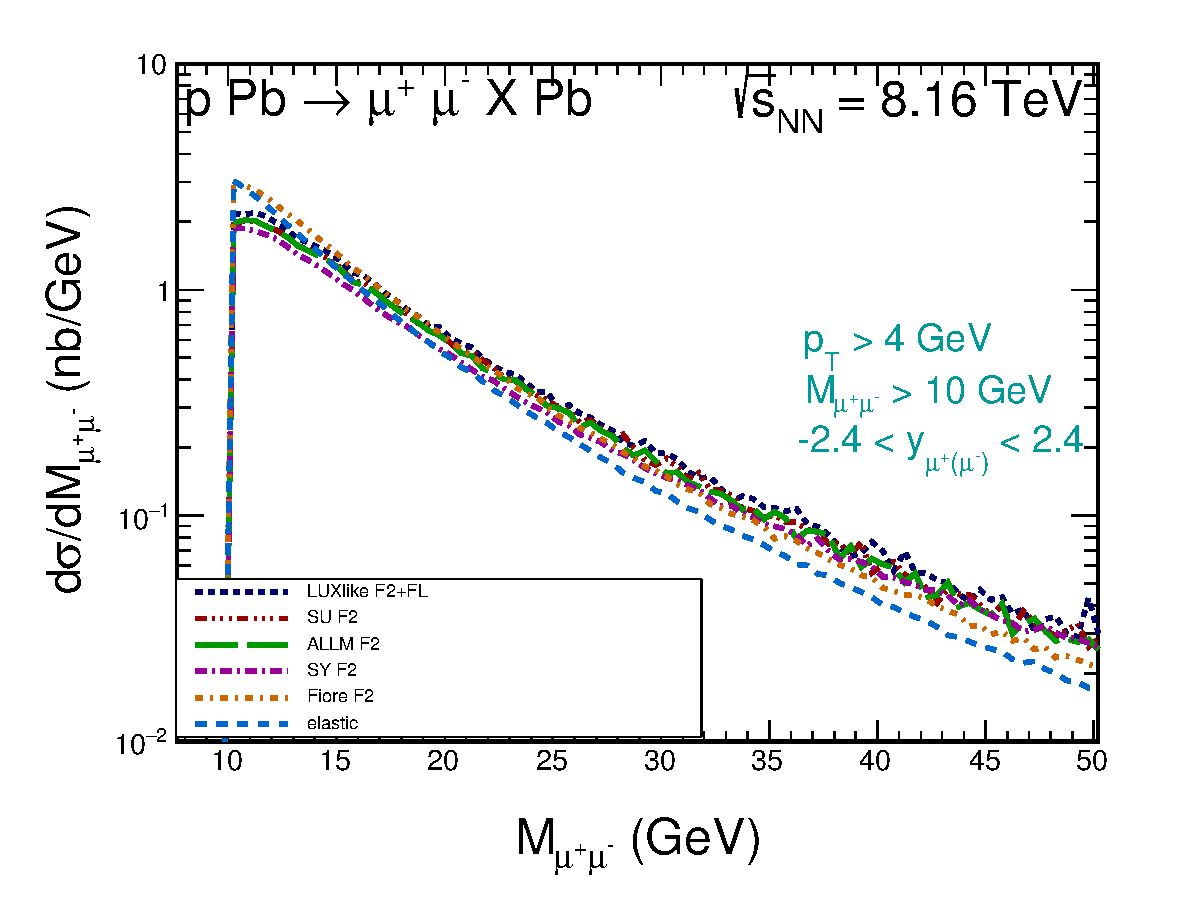
\includegraphics[width=0.49\textwidth]{figures_Marta/Mll-c.pdf}
  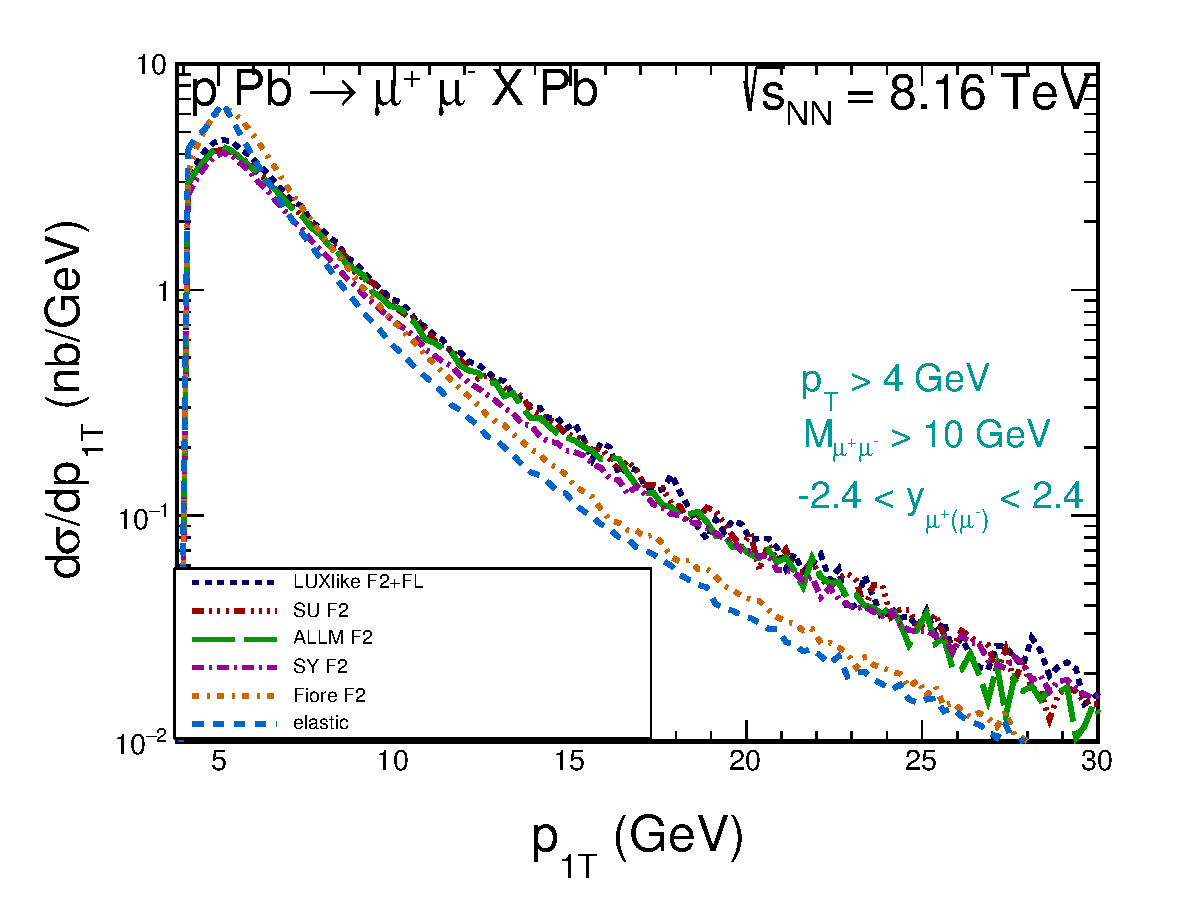
\includegraphics[width=0.49\textwidth]{figures_Marta/pt1-c.pdf}
 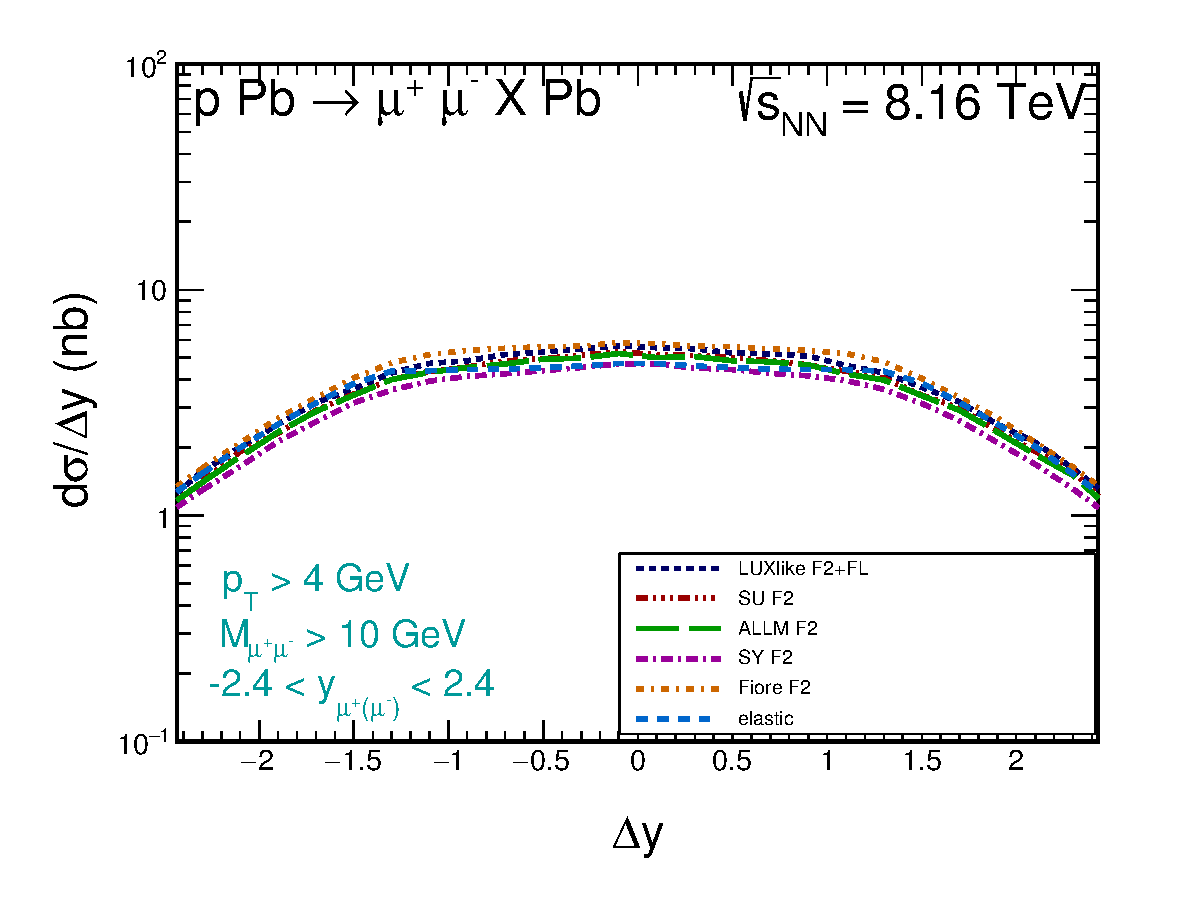
\includegraphics[width=0.49\textwidth]{figures_Marta/ydiff-c.pdf}
  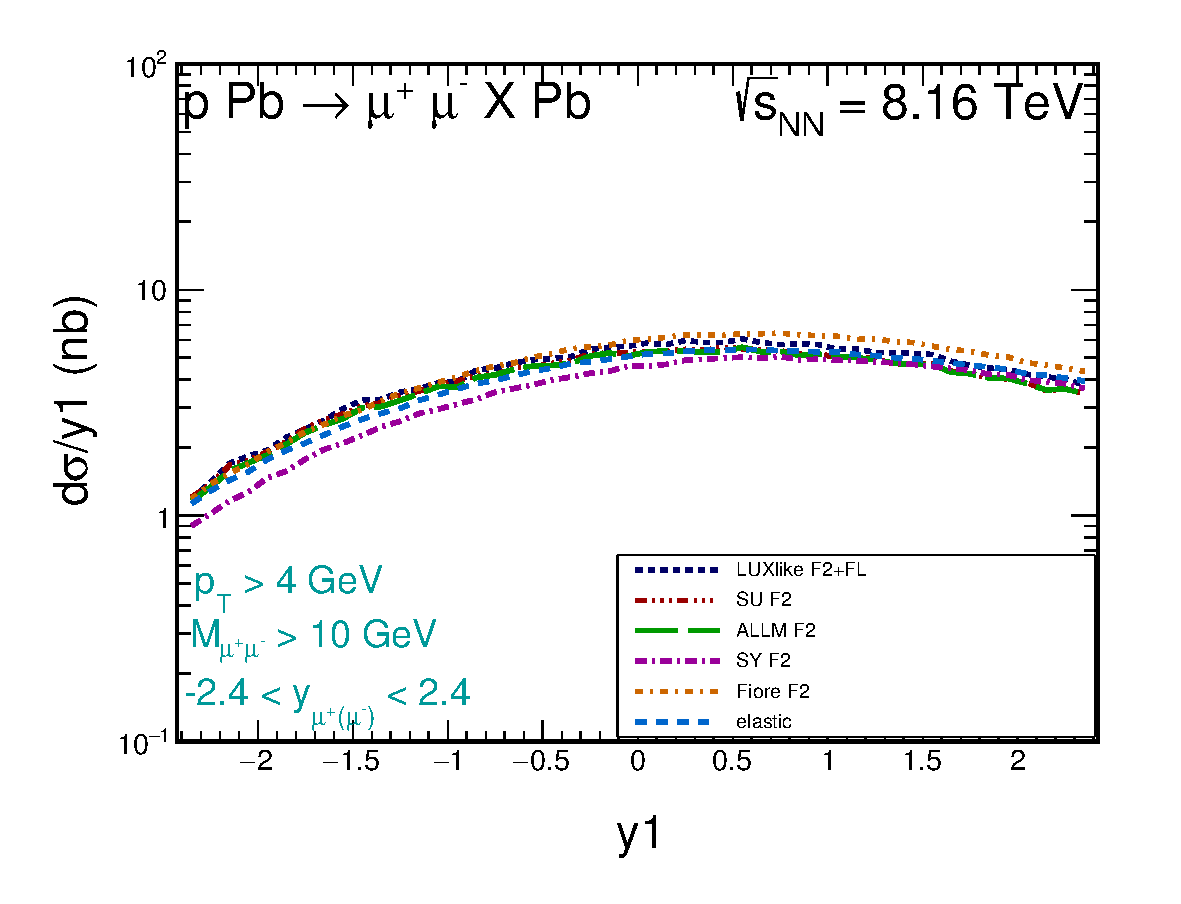
\includegraphics[width=0.49\textwidth]{figures_Marta/y1-c.pdf}
\caption{Differential cross sections in the fiducial region for $p+\textrm{Pb}\rightarrow \textrm{Pb} + \ell^+\ell^- + X$ production at $\sqrt{s_{N N}} = 8.16$~\TeV\ in $k_T$ factorization approach for several proton structure functions.
Four differential distributions are shown: invariant mass of lepton pair (top left), leading lepton transverse momentum (top right),
lepton pseudorapidity difference (bottom left) and leading lepton pseudorapidity (bottom right).
For comparison, the elastic contribution ($p+\textrm{Pb}\rightarrow p+ \textrm{Pb} + \ell^+\ell^-$) is also shown.
}
 \label{fig:kt_figures1}
\end{figure}
%------------------------------------------------------------------------------


%-----------------------------------------------------------------------------
\begin{figure}[!h]
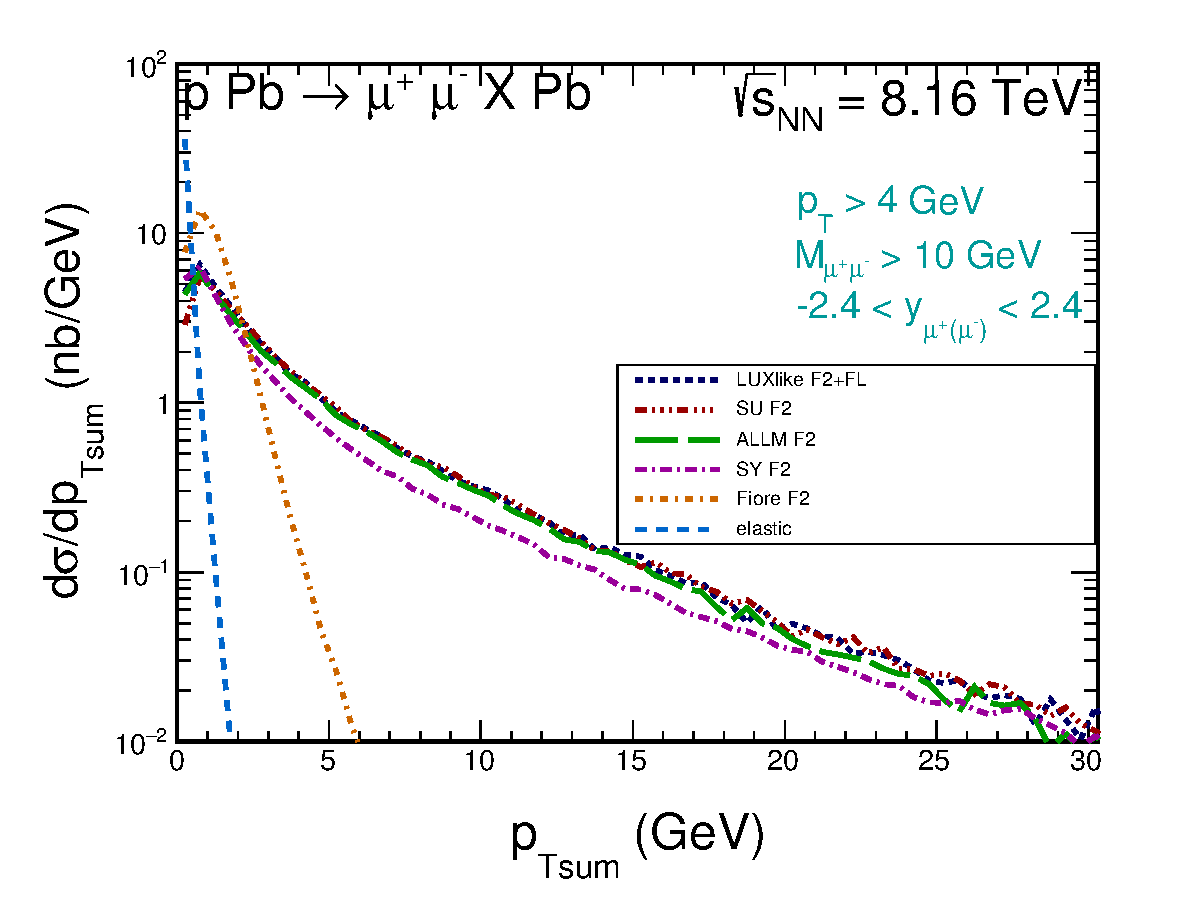
\includegraphics[width=0.49\textwidth]{figures_Marta/ptsum-c.pdf}
 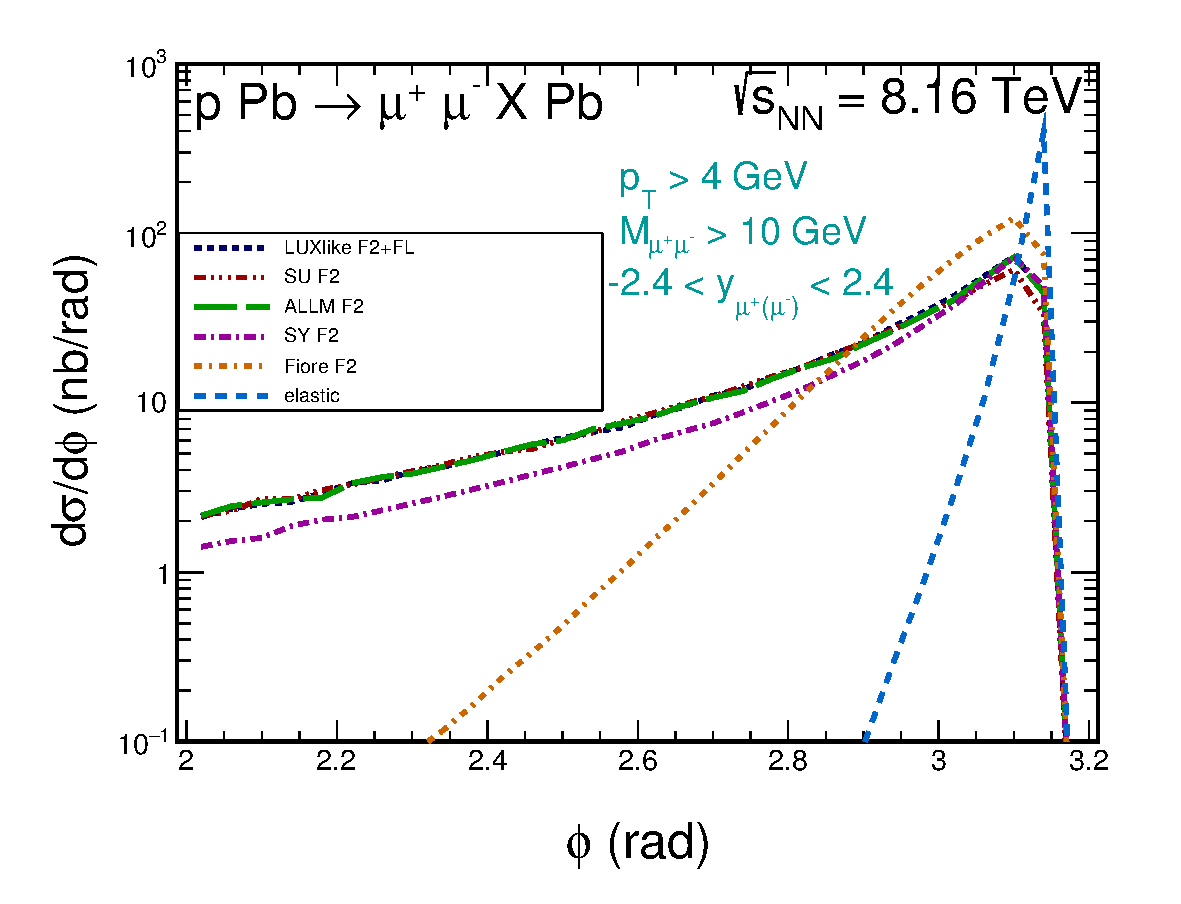
\includegraphics[width=0.49\textwidth]{figures_Marta/phi-c.pdf}
\caption{Differential cross sections in the fiducial region for $p+\textrm{Pb}\rightarrow \textrm{Pb} + \ell^+\ell^- + X$ production at $\sqrt{s_{N N}} = 8.16$~\TeV\ in $k_T$ factorization approach for several proton structure functions.
Two differential distributions are shown: transverse momentum of lepton pair (left) and azimuthal angle difference between the pair (right).
For comparison, the elastic contribution ($p+\textrm{Pb}\rightarrow p+ \textrm{Pb} + \ell^+\ell^-$) is also shown.
}
 \label{fig:kt_figures2}
\end{figure}
%------------------------------------------------------------------------------


%-----------------------------------------------------------------------------
\begin{figure}[!h]

 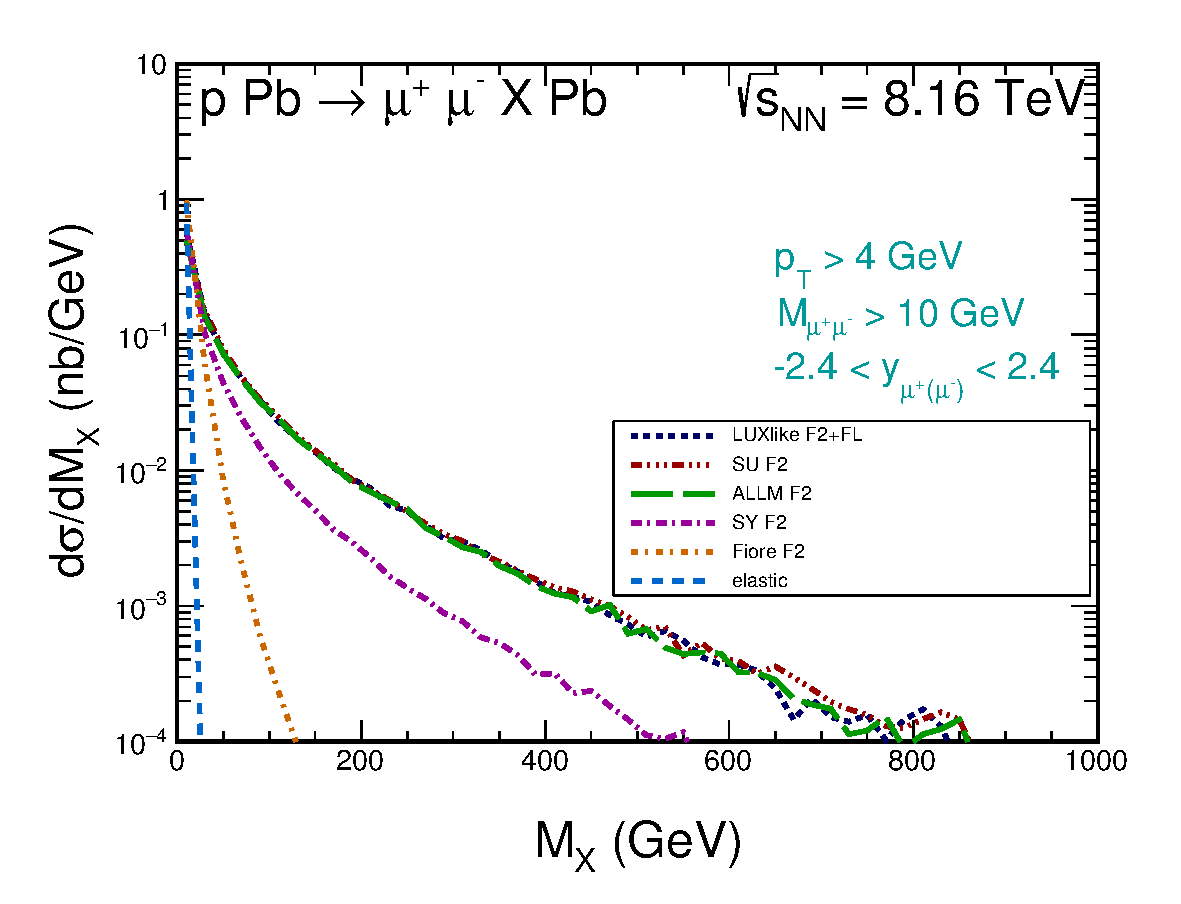
\includegraphics[width=0.49\textwidth]{figures_Marta/MX-c.pdf}
\caption{Differential cross section as a function of the mass of the proton remnants in the fiducial region for $p+\textrm{Pb}\rightarrow \textrm{Pb} + \ell^+\ell^- + X$ production at $\sqrt{s_{N N}} = 8.16$~\TeV\ in $k_T$ factorization approach for several proton structure functions.
For comparison, the elastic contribution ($p+\textrm{Pb}\rightarrow p+ \textrm{Pb} + \ell^+\ell^-$) is also shown.
}
 \label{fig:kt_figures3}
\end{figure}
%------------------------------------------------------------------------------





%
%%-----------------------------------------------------------------------------
%\begin{figure}[!h]
%\begin{minipage}{0.47\textwidth}
% \centerline{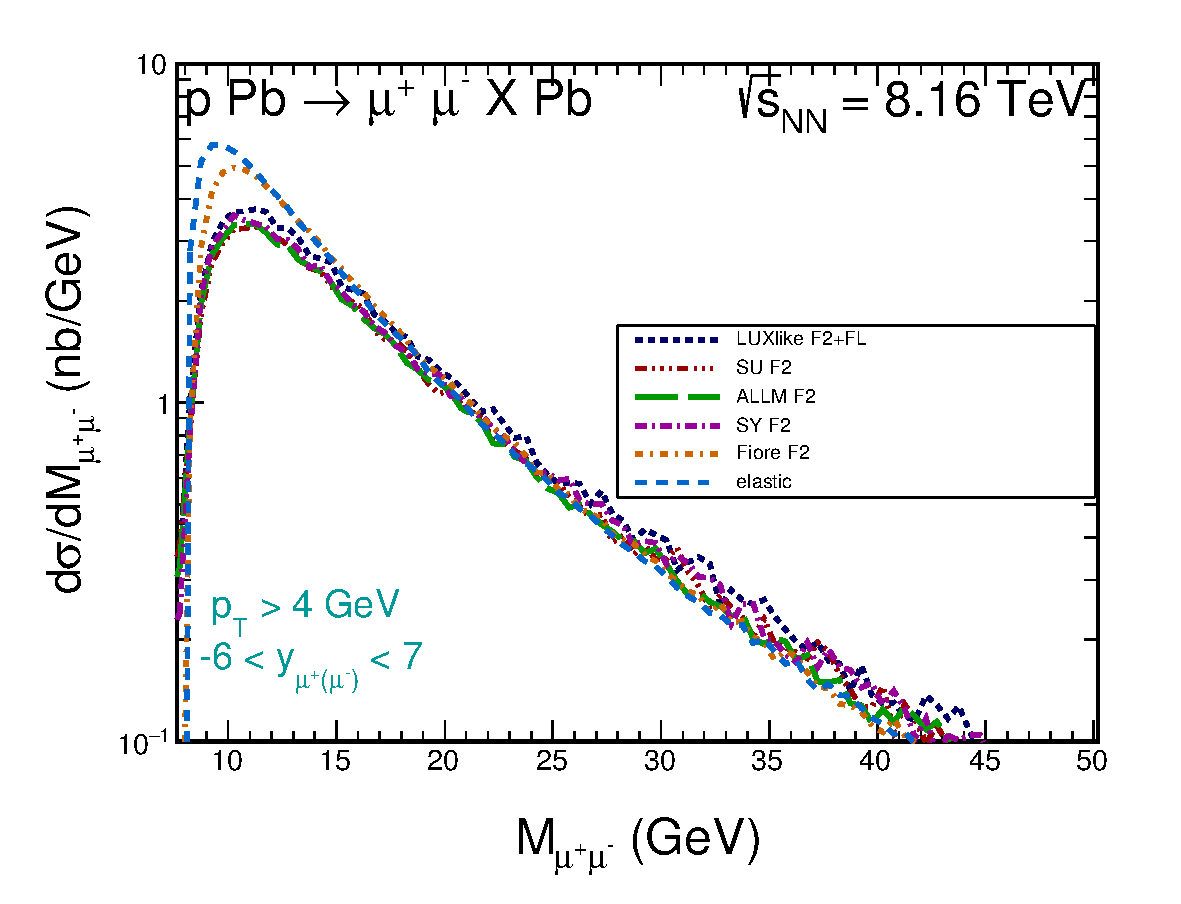
\includegraphics[width=1.0\textwidth]{figures_Marta/Mll.pdf}}
%\end{minipage}
%\begin{minipage}{0.47\textwidth}
% \centerline{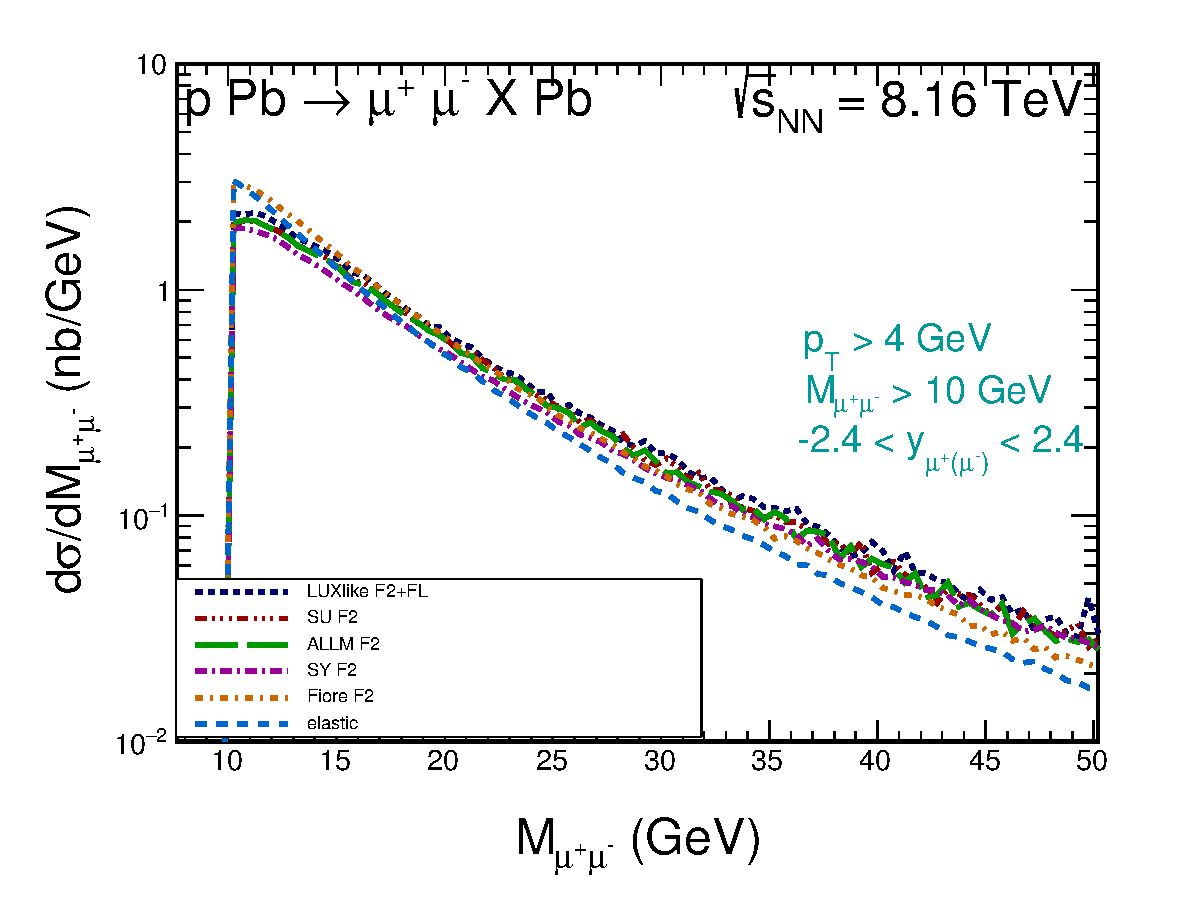
\includegraphics[width=1.0\textwidth]{figures_Marta/Mll-c.pdf}}
%\end{minipage}
%\caption{The elastic - elastic and the inelastic-elastic contribution 
%to dilepton invariant mass distributions 
%for different structure functions. In the left panel we show the results for the whole phase space, while in the right panel only for the fiducial region.
%}
% \label{fig:dsig_dMWW_ineine}
%\end{figure}
%%------------------------------------------------------------------------------
%
%%-----------------------------------------------------------------------------
%\begin{figure}[!htbp]
%\begin{minipage}{0.47\textwidth}
% \centerline{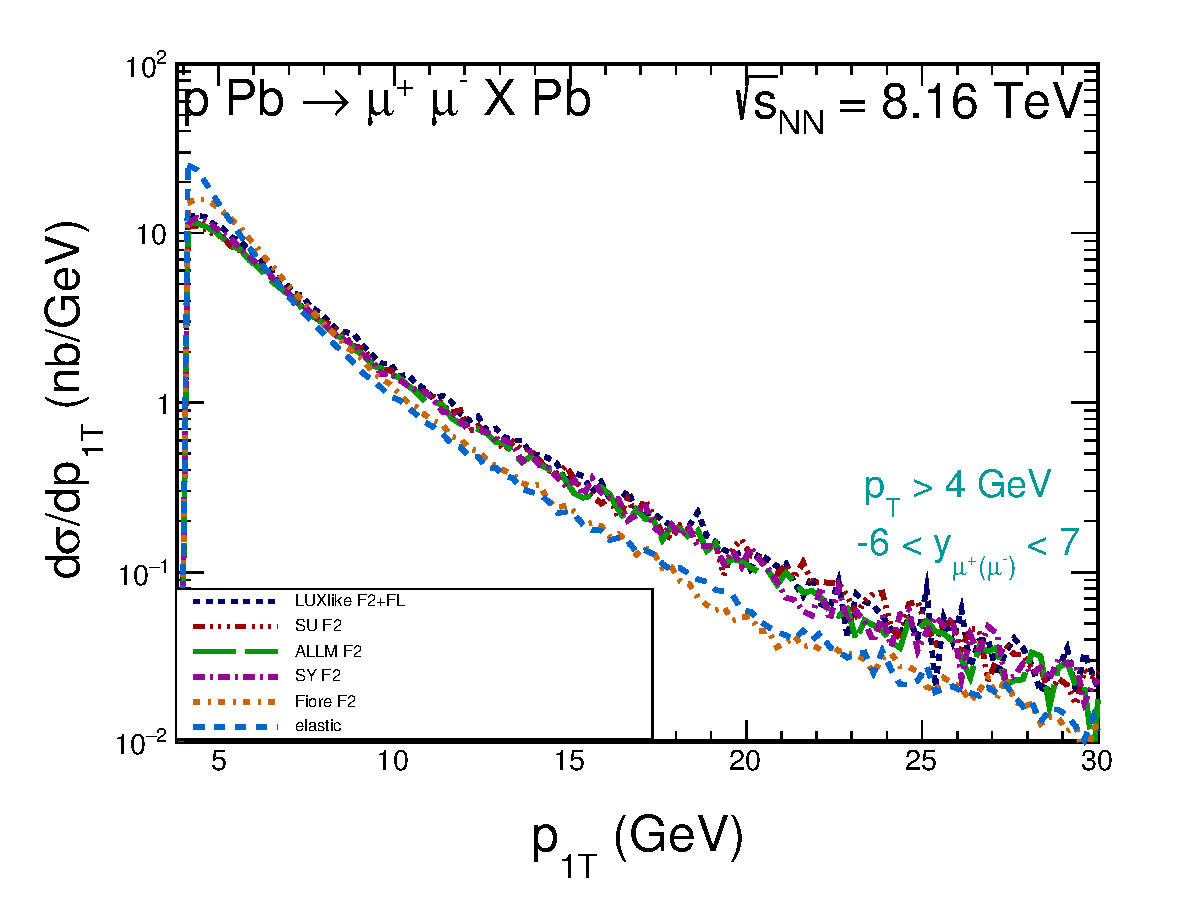
\includegraphics[width=1.0\textwidth]{figures_Marta/pt1.pdf}}
%\end{minipage}
%\begin{minipage}{0.47\textwidth}
% \centerline{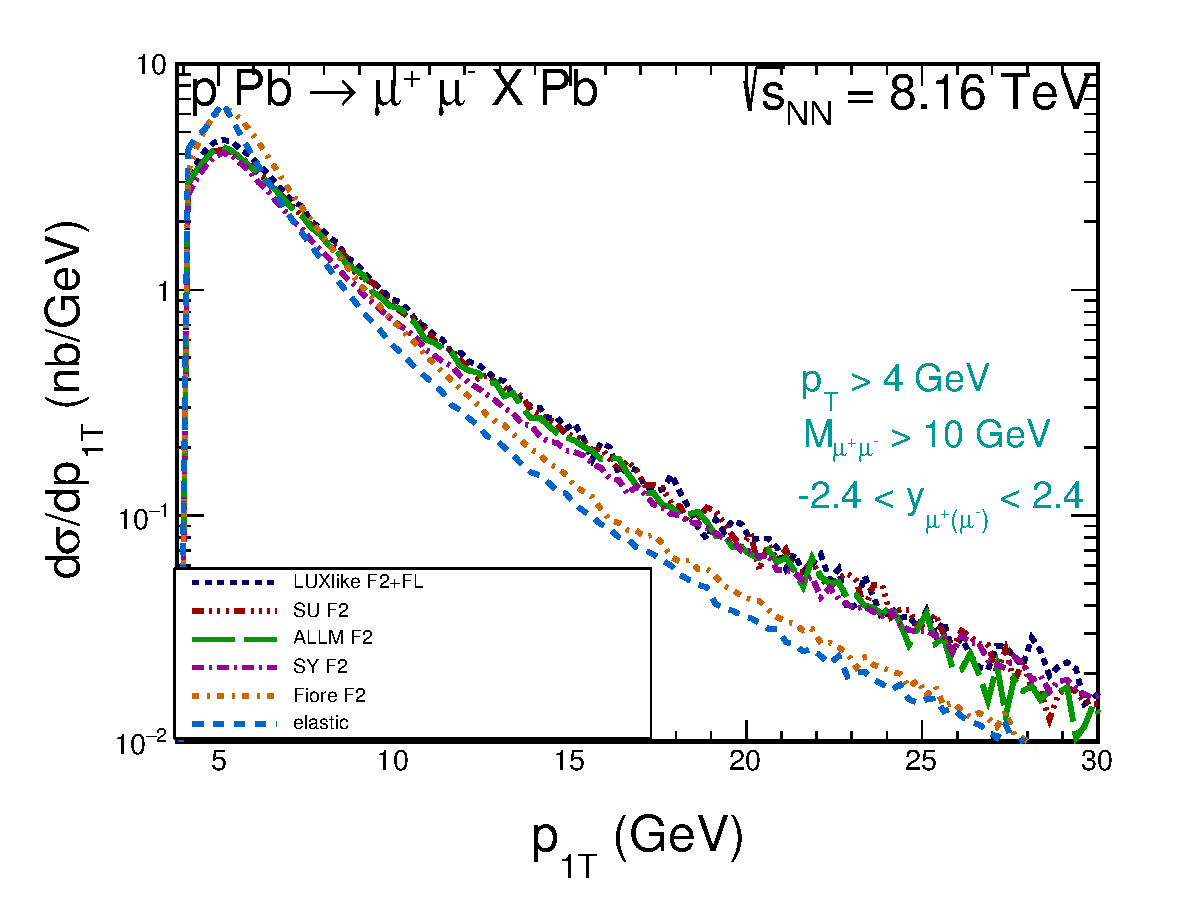
\includegraphics[width=1.0\textwidth]{figures_Marta/pt1-c.pdf}}
%\end{minipage}
%\caption{
%Transverse momentum distribution of $\mu^+$ or $\mu^-$ 
%for elastic - elastic and inelastic - elastic different structure functions: LUX-like, ALLM97, Fiore at all., SU and SY (in the left panel we show the results for the whole phase space, while in the right panel only for the fiducial region).
%}
% \label{fig:dsig_dMWW_ineine}
%\end{figure}
%%------------------------------------------------------------------------------
%
%
%%-----------------------------------------------------------------------------
%\begin{figure}[!htbp]
%\begin{minipage}{0.47\textwidth}
% \centerline{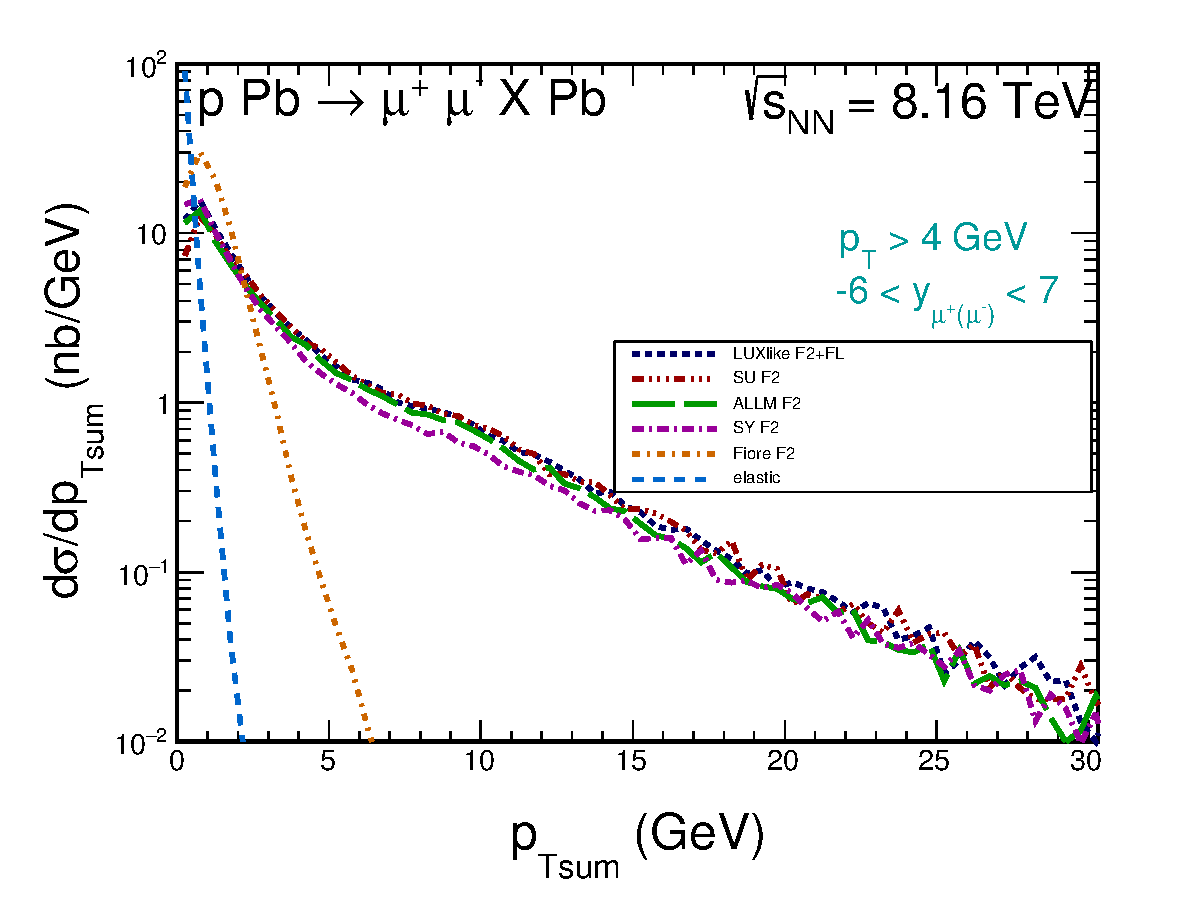
\includegraphics[width=1.0\textwidth]{figures_Marta/ptsum.pdf}}
%\end{minipage}
%\begin{minipage}{0.47\textwidth}
% \centerline{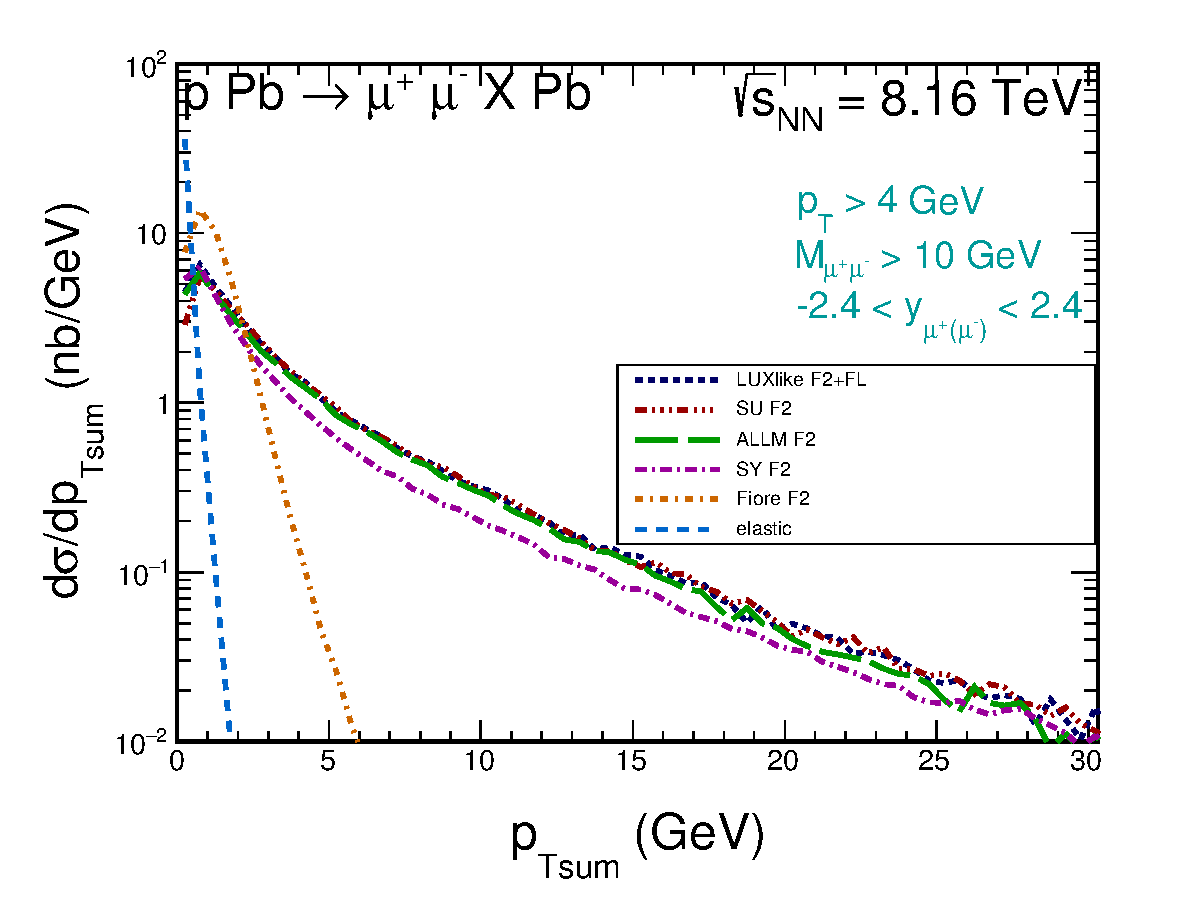
\includegraphics[width=1.0\textwidth]{figures_Marta/ptsum-c.pdf}}
%\end{minipage}
%\caption{
%Distribution in transverse momentum of the $\mu^+ \mu^-$ pairs for elastic - elastic and 
%inelastic-elastic
%contributions
%for different structure functions: LUX-like, ALLM97, Fiore at all., SU and SY. (in the left panel we show the results for the whole phase space, while in the right panel only for the fiducial region).
%}
% \label{fig:dsig_dMWW_ineine}
%\end{figure}
%%------------------------------------------------------------------------------
%
%
%%-----------------------------------------------------------------------------
%\begin{figure}[!htbp]
%\begin{minipage}{0.47\textwidth}
% \centerline{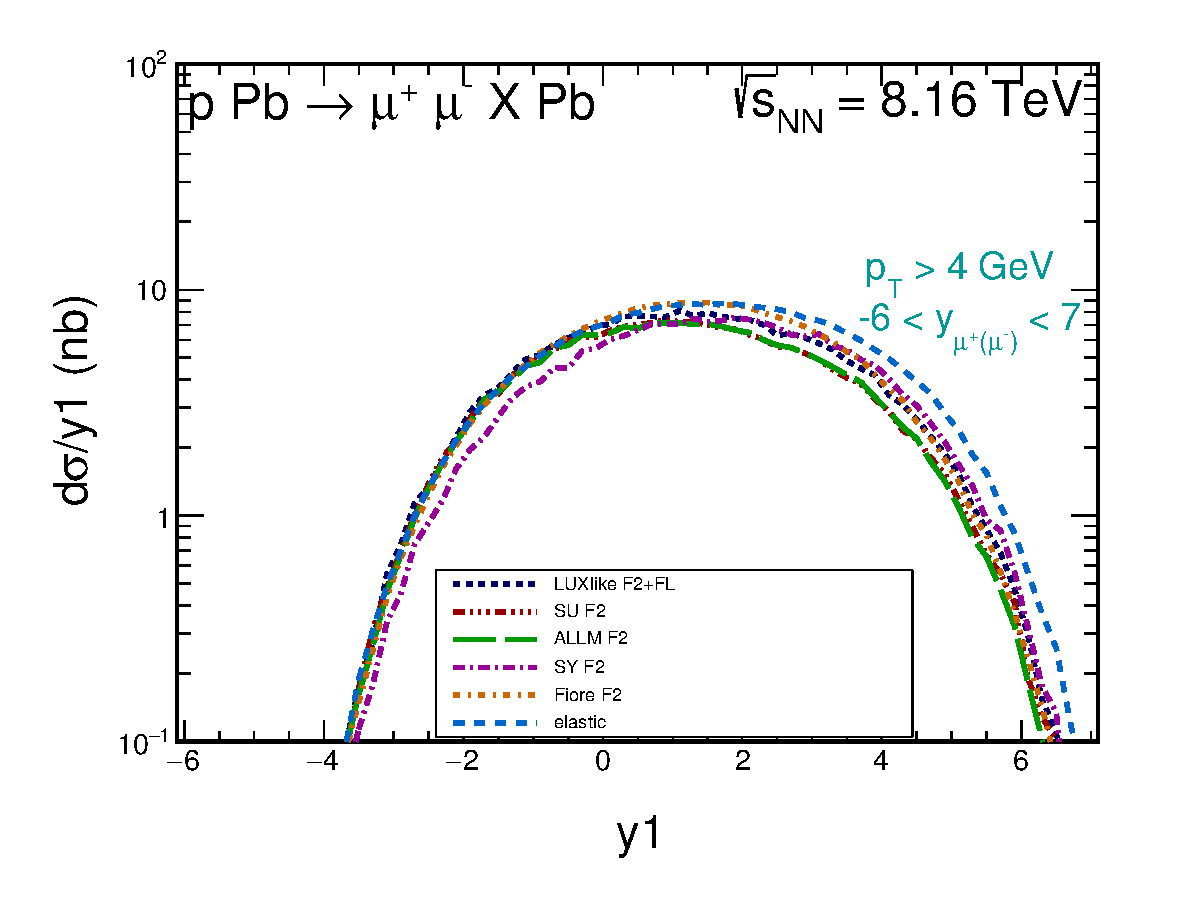
\includegraphics[width=1.0\textwidth]{figures_Marta/y1.pdf}}
%\end{minipage}
%\begin{minipage}{0.47\textwidth}
% \centerline{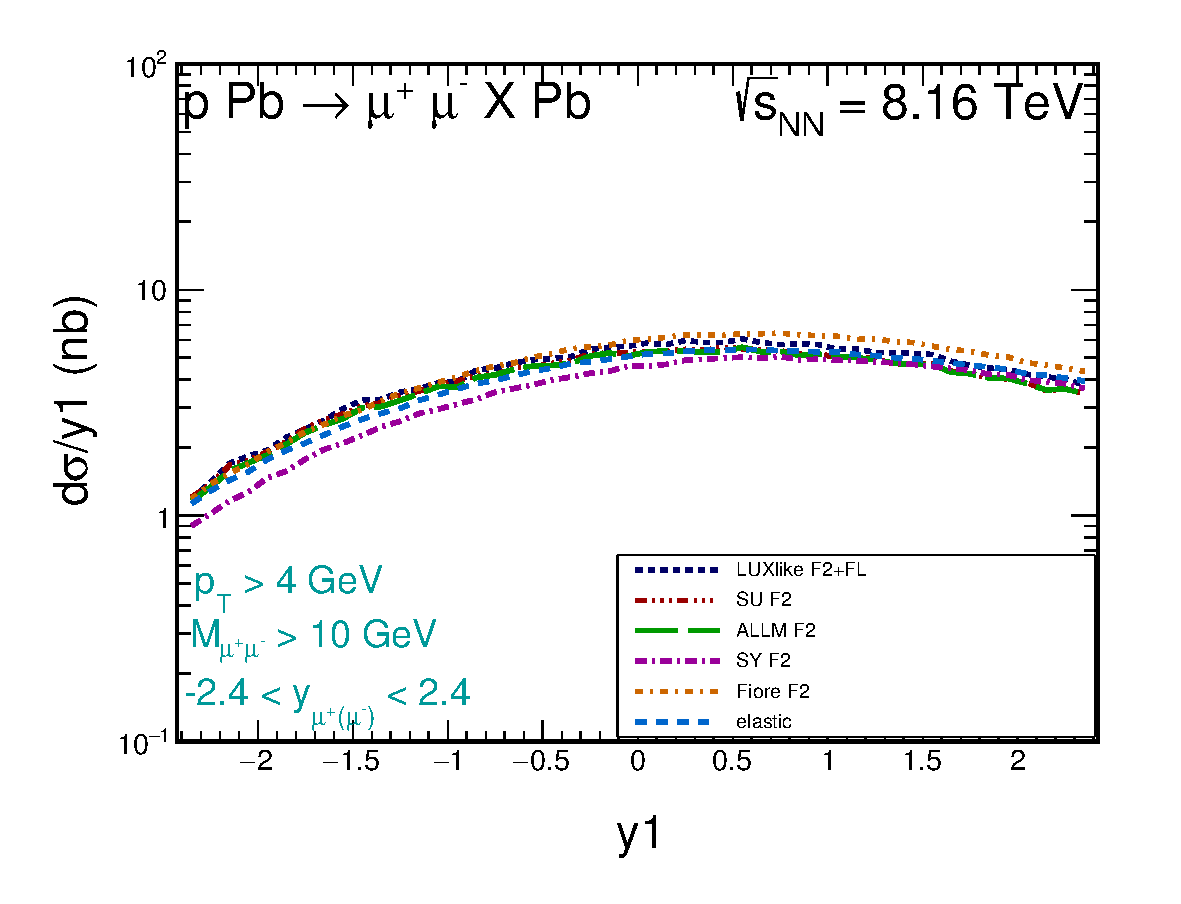
\includegraphics[width=1.0\textwidth]{figures_Marta/y1-c.pdf}}
%\end{minipage}
%
%\caption{
%Rapidity distribution of $\mu^+$ or $\mu^-$ leptons
%for elastic - elastic and inelastic-elastic contributions for different structure functions: LUX-like, ALLM97, Fiore at all., SU and SY. (in the left panel we show the results for the whole phase space, while in the right panel only for the fiducial region).
%}
% \label{fig:dsig_dMWW_ineine}
%\end{figure}
%%------------------------------------------------------------------------------
%
%
%
%%------------------------------------------------------------------------------
%
%%-----------------------------------------------------------------------------
%\begin{figure}[!htbp]
%\begin{minipage}{0.47\textwidth}
% \centerline{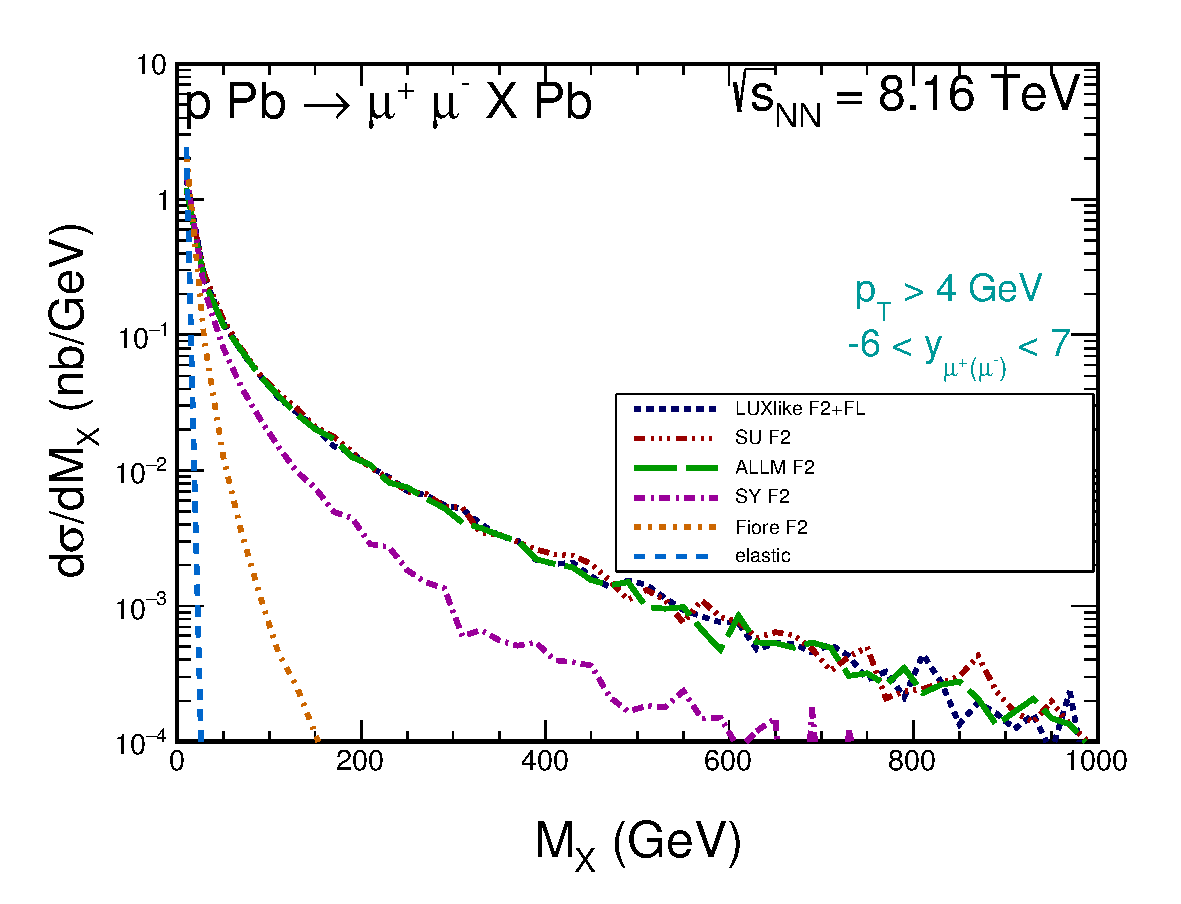
\includegraphics[width=1.0\textwidth]{figures_Marta/MX.pdf}}
%\end{minipage}
%%\hspace{0.5cm}
%\begin{minipage}{0.47\textwidth}
% \centerline{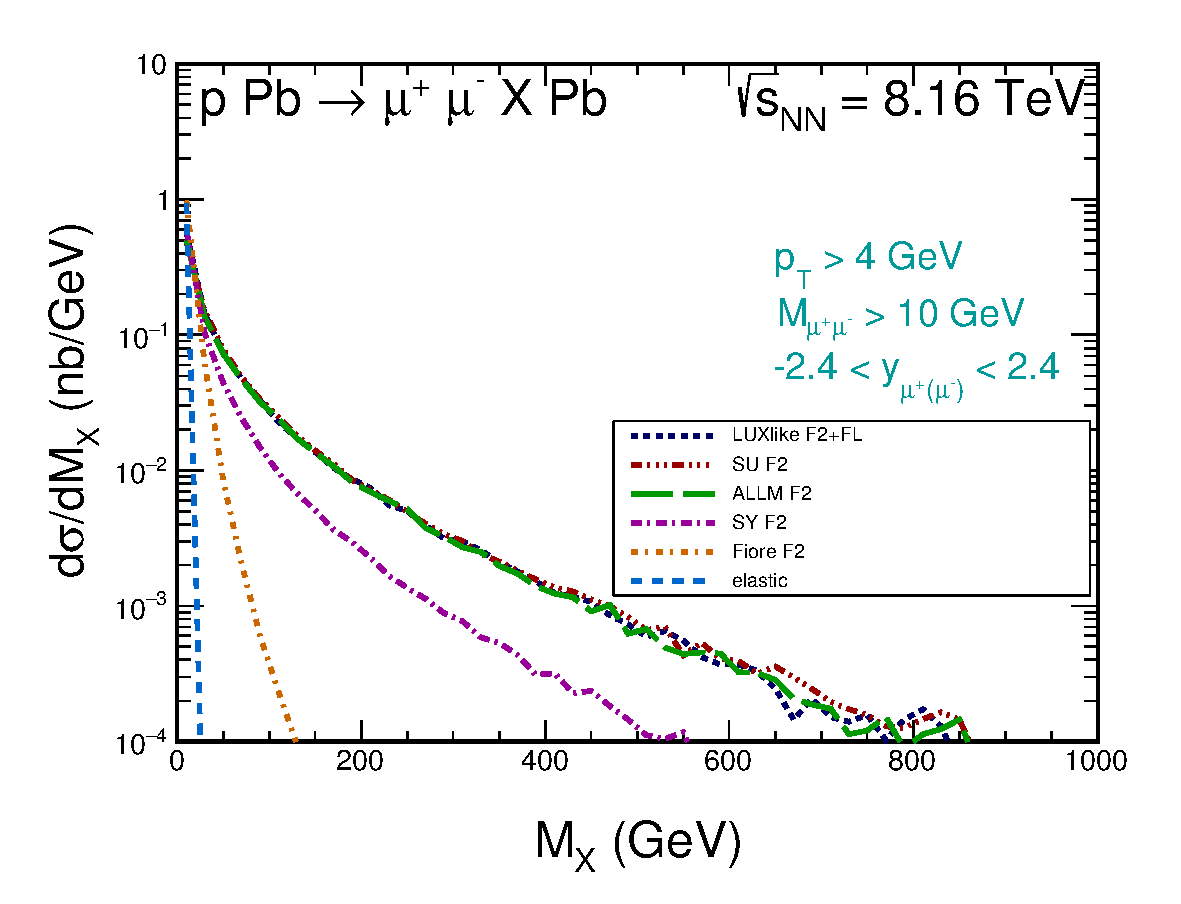
\includegraphics[width=1.0\textwidth]{figures_Marta/MX-c.pdf}}
%\end{minipage}
%\caption{
%Missing mass distributions for eleastic-elastic photon-photon contributions and elastic-inelastic photon-photon contributions for different structure functions: LUX-like, ALLM97, Fiore at all., SU and SY. (in the left panel we show the results for the whole phase space, while in the right panel only for the fiducial region).
%}
%\label{fig:dsig_dy}
%\end{figure}
%%---------------------------------------------------------------
%
%
%
%
%%-----------------------------------------------------------------------------
%\begin{figure}[!htbp]
%\begin{minipage}{0.47\textwidth}
% \centerline{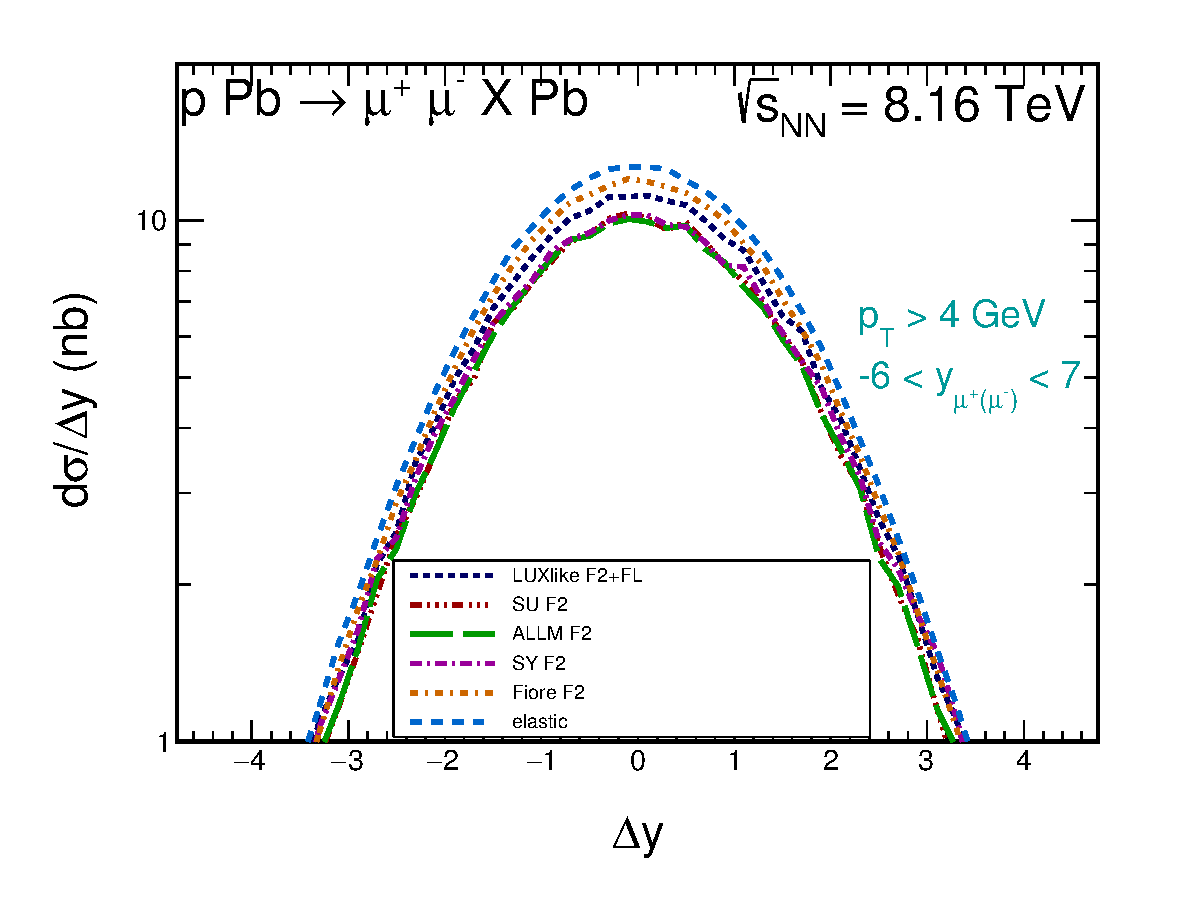
\includegraphics[width=1.0\textwidth]{figures_Marta/ydiff.pdf}}
%\end{minipage}
%%\hspace{0.5cm}
%\begin{minipage}{0.47\textwidth}
% \centerline{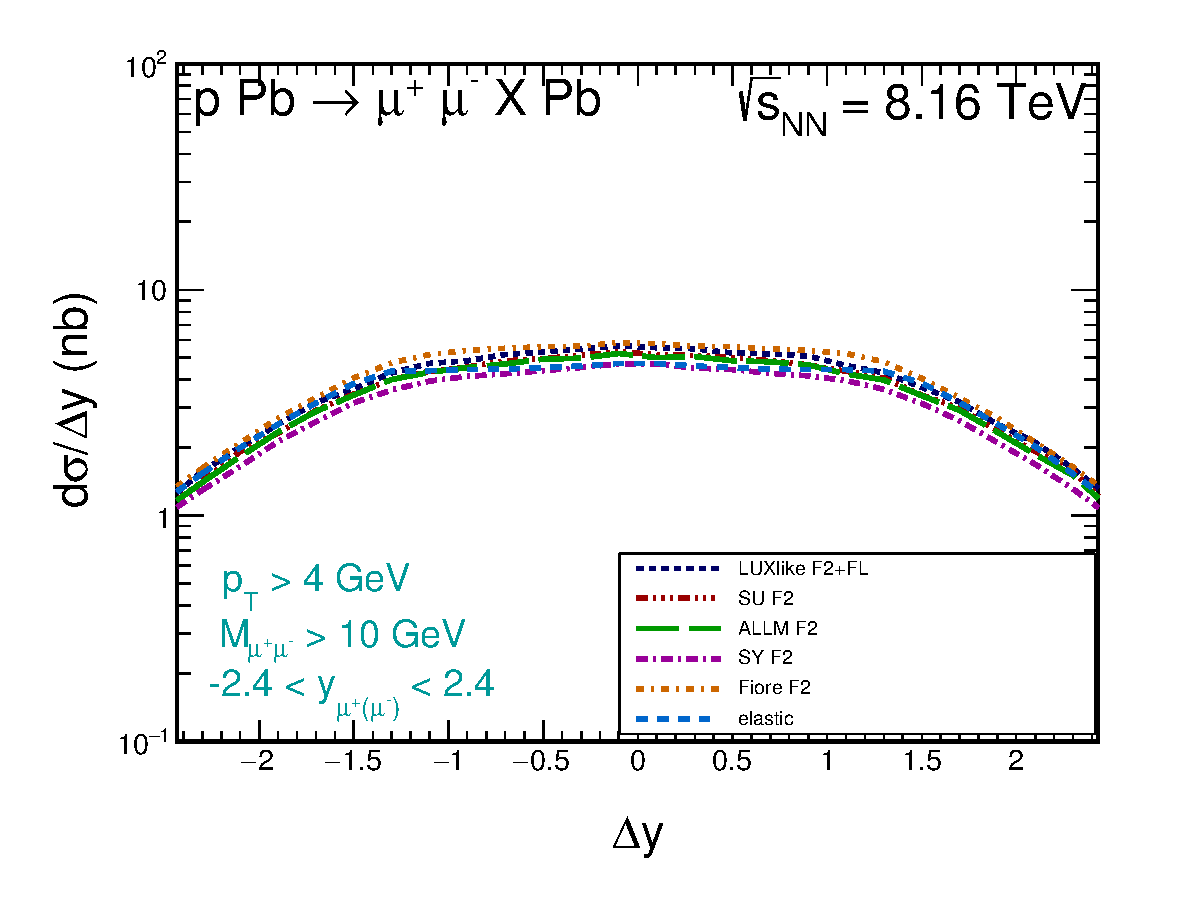
\includegraphics[width=1.0\textwidth]{figures_Marta/ydiff-c.pdf}}
%\end{minipage}
%\caption{
%Distribution in rapidity distance between $\mu^+\mu^-$ leptons.
%The calculation for the $\gamma-\gamma$ contribution
%was performed for different structure functions. 
%The left panel shows results  without cuts while the right panel 
%shows results with ATLAS cuts.
%}
%\label{fig:dsig_dy}
%\end{figure}
%%---------------------------------------------------------------
%
%%-----------------------------------------------------------------------------
%\begin{figure}[!htbp]
%\begin{minipage}{0.47\textwidth}
% \centerline{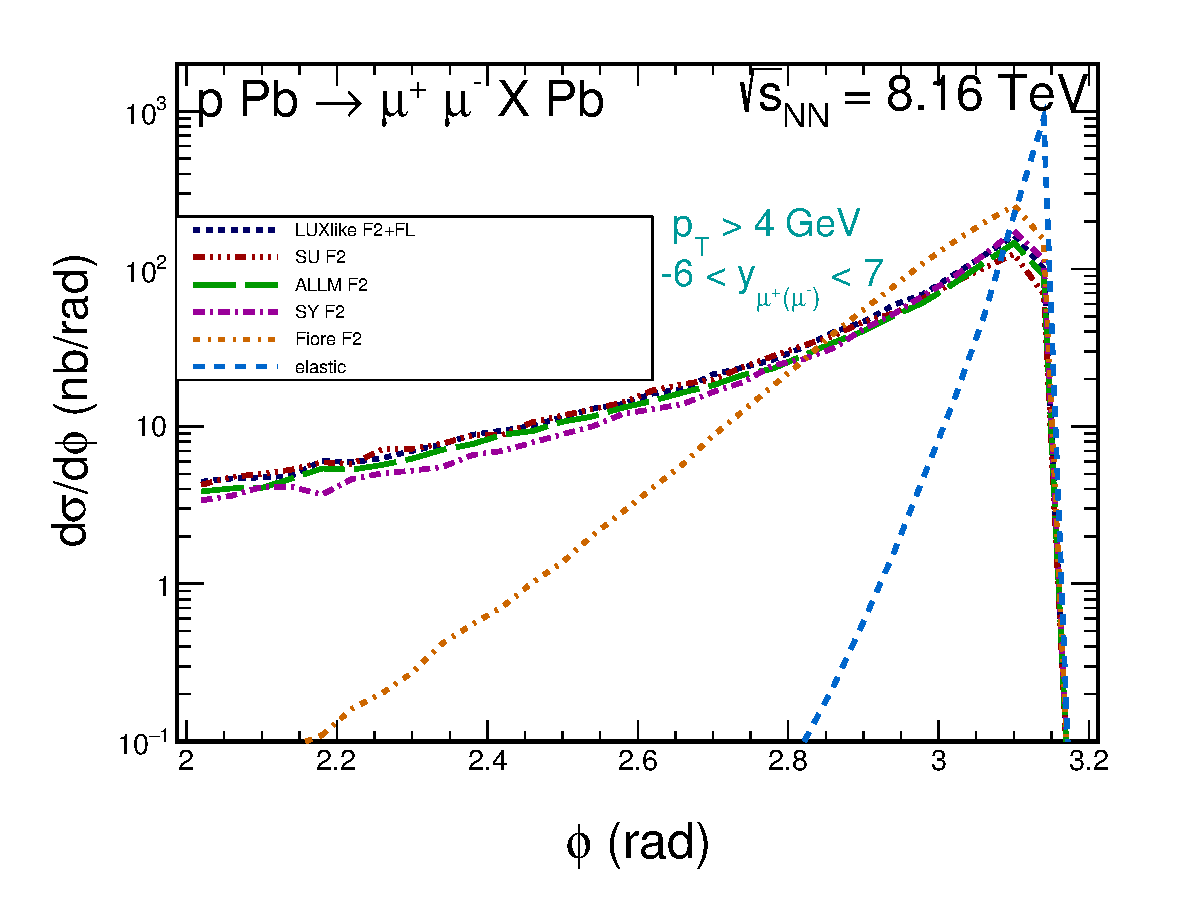
\includegraphics[width=1.0\textwidth]{figures_Marta/phi.pdf}}
%\end{minipage}
%%\hspace{0.5cm}
%\begin{minipage}{0.47\textwidth}
% \centerline{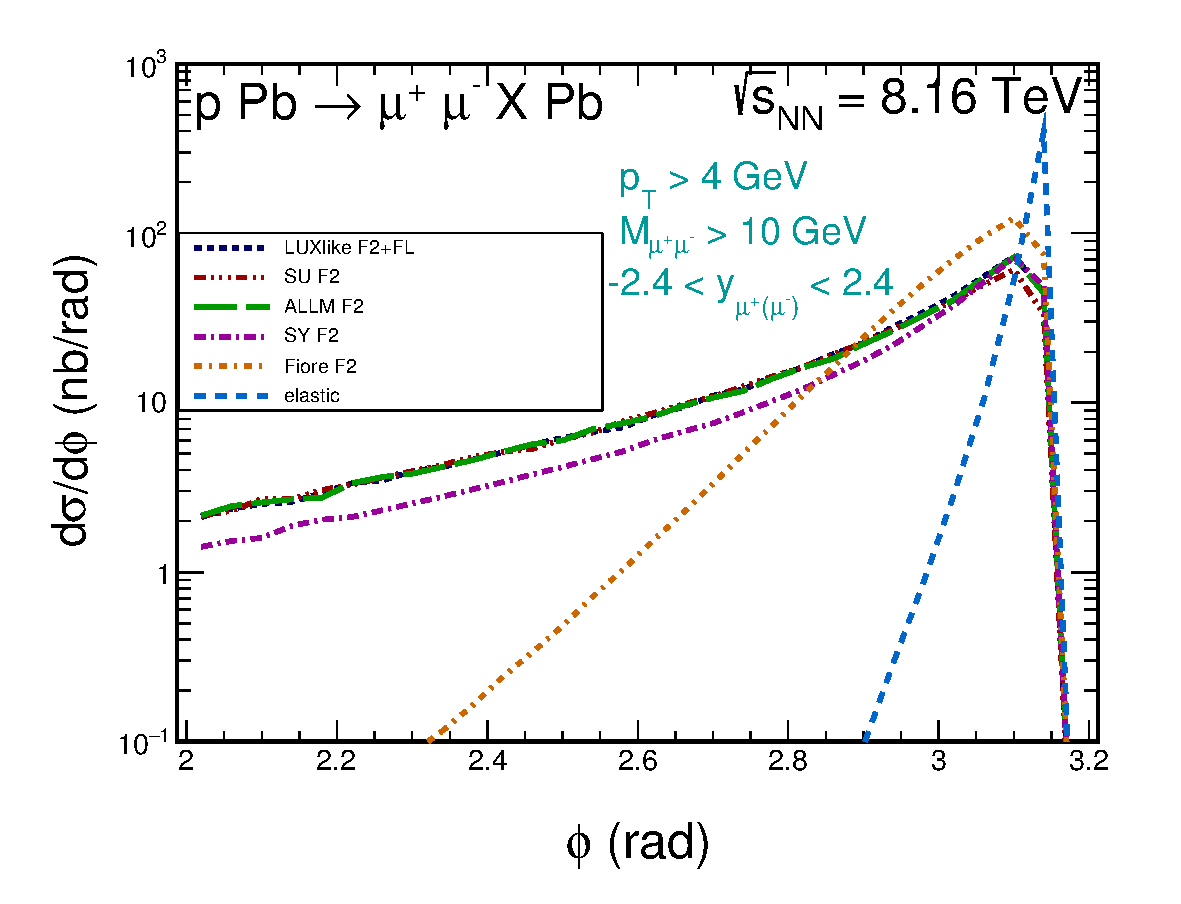
\includegraphics[width=1.0\textwidth]{figures_Marta/phi-c.pdf}}
%\end{minipage}
%\caption{
%Distributions for azimuthal angle between $\mu^+\mu^-$ leptons. (in the left panel we show the results for the whole phase space, while in the right panel only for the fiducial region).
%}
%\label{fig:dsig_dy}
%\end{figure}
%%---------------------------------------------------------------




